\documentclass[a4paper,11pt]{jsarticle}

% パッケージ
\usepackage[dvipdfmx]{hyperref}
\usepackage{pxjahyper}
\usepackage[dvipdfmx]{graphicx}
\usepackage{ascmac}
\usepackage{fancybox}
\usepackage{listings}
\usepackage{plistings}
\usepackage{multirow}
\usepackage[subrefformat=parens]{subcaption}
\usepackage{color}
\usepackage{here}
\usepackage{subcaption}
\usepackage{longtable}
\usepackage{amsmath,amsfonts}
\usepackage[utf8]{inputenc}
\usepackage{bm}
\usepackage{siunitx}
\usepackage{url}
% ページの周りの余白
\usepackage[top=25truemm,bottom=25truemm,left=30truemm,right=30truemm]{geometry}

% URLの設定
\Urlmuskip=0mu  plus 10mu

% 色の定義
\definecolor{OliveGreen}{rgb}{0.0,0.6,0.0}
\definecolor{Magenta}{cmyk}{0, 1, 0, 0}
\definecolor{colFunc}{rgb}{1,0.07,0.54}
\definecolor{CadetBlue}{cmyk}{0.62,0.57,0.23,0}
\definecolor{Brown}{cmyk}{0,0.81,1,0.60}
\definecolor{colID}{rgb}{0.63,0.44,0}


\lstset{
  basicstyle={\ttfamily},
  identifierstyle={\small},
  commentstyle={\smallitshape},
  keywordstyle={\small\bfseries},
  ndkeywordstyle={\small},
  stringstyle={\small\ttfamily},
  frame={tb},
  breaklines=true,
  columns=[l]{fullflexible},
  numbers=left,
  xrightmargin=0zw,
  xleftmargin=3zw,
  numberstyle={\scriptsize},
  stepnumber=1,
  numbersep=1zw,
  lineskip=-0.5ex
}

\renewcommand{\lstlistingname}{Code}

% リンクの設定
\hypersetup{
  setpagesize=false,
  bookmarksnumbered=true,
  bookmarksopen=true,
  colorlinks=true,
  linkcolor=blue,
  citecolor=red,
}

\begin{document}

%\title{}
%\author{}
%\date{\today}
%\maketitle


\section{目的}
三年次の制御情報システム工学演習で,PLCシーケンス制御について学習した.今日では一般の工場でラインの自動化に広く使われており,
IoTやスマートファクトリーの土台になっている.\par
「機械を制御する」目的に使用されるPLCに直接触れ,簡単な動作を行うことでPLCについての基礎知識を身につける.
また,回路作成,プログラムの作成をチームで行うことにより,協力して問題解決をする能力を身に付けることを本実験の目的とする.

\section{理論}
\subsection{PLCとは}
PLCとは,機械を自動的に制御する装置であり,正式名称はProgrammable Logic Controller(プログラマブルロジックコントローラ)
である.PLCは「シーケンス制御」という考え方のもと動作する.シーケンス制御について,日本工業規格(JIS)は以下のように定義している.~\cite{JIS}
\begin{quote}
  あらかじめ定められた順序又は手続きに従って制御の各段階を逐次進めていく制御。
\end{quote}
PLCを用いることによるメリットには以下のようなことが挙げられる.
\begin{itemize}
  \item 小型なため,省スペース \\
        リレーの配線が不要であることや,比較的コンパクトな設計であるため,設置スペースを小さくすることができる.工場では,多くの機械,装置を配置する必要があるため,省スペースで機械の制御ができることは大きなメリットとなる.
  \item 動作の変更が容易\\
        PLCはプログラミング言語を用いて機械を制御する.有接点シーケンス制御方式を採用していると,動作の変更をするたびに電気部品を付け替えたり,配線の見直しをおこなったりと,面倒なことが多い.しかし,PLCはプログラムを変更するだけで容易に動作を変更することができるため,手間を省くことができる.
\end{itemize}


\section{実験方法}
実験については,授業資料~\cite{Text}を参考にする.STEP10~STEP12について,資料を参考にしながら回路を設計し,CX-programmerを利用して,ラダー図を作成する.
有線ケーブルを用いて,実験ボード上にあるPLCに送信して動作を確認する.
\subsection{STEP10}
\subsubsection{理想動作}
押しボタンスイッチ1をONすると,ONの間モータ1は右移動し,モータ2は右回転します.\\
押しボタンスイッチ2をONすると,モータ1だけが左移動します.\par
なお,押しボタンスイッチ1がONの間は押しボタンスイッチ2の入力を遮断し,押しボタンスイッチ2がONの間は
押しボタンスイッチ1の入力を遮断するというインターロック回路が設けてあります.

\subsection{STEP11}
\subsubsection{理想動作}
押しボタンスイッチ1をONすると,モータ1が正回転(右移動)します.モータ1の移動によってLS2(センサ)がONになると,
モータ1は停止します,1秒間停止後,再び正回転を始め,LS3がONになると,モータ1は0.5秒間停止します.その後今度は
逆回転(左移動)を始め,LS1がONになるとモータ1は停止します.再度押しボタンスイッチ1をONにすると,同じ動作を繰り返します.

\section{実験環境}
実験に使用したソフトと,動作環境を以下の表\ref{T:En}に示す.
\begin{table}[H]
  \begin{center}
    \caption{実験環境}
    \begin{tabular}{|c|c|} \hline
      ソフトウェア & CX-programmer             \\ \hline
      OS           & Windows7                  \\ \hline
      ボード       & アイディープロ MS4-000-Vt \\ \hline
      PLC          & omron SYSMAC CP1L         \\ \hline
    \end{tabular}
    \label{T:En}
  \end{center}
\end{table}

\section{実験結果}
\subsection{STEP10}
以下の図\ref{P:Circuit10}に作成した回路図を示し,図\ref{C:Step10}に作成したラダー図を示す.
\begin{figure}[H]
  \begin{minipage}{0.38\textwidth}
    \begin{center}
      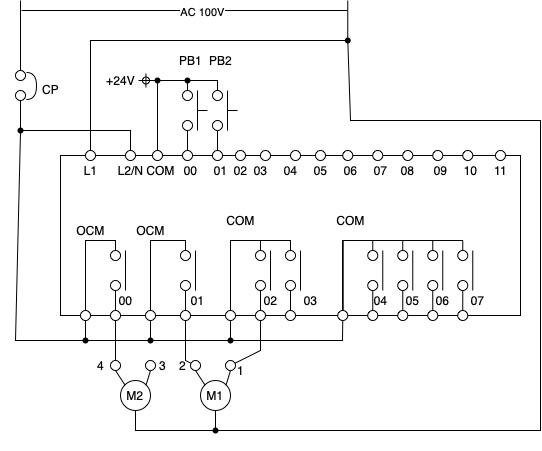
\includegraphics[clip,width=6.5cm]{picture/Circuit10.png}
    \end{center}
    \caption{STEP10の回路図}
    \label{P:Circuit10}
  \end{minipage}
  \begin{minipage}{0.58\textwidth}
    \begin{center}
      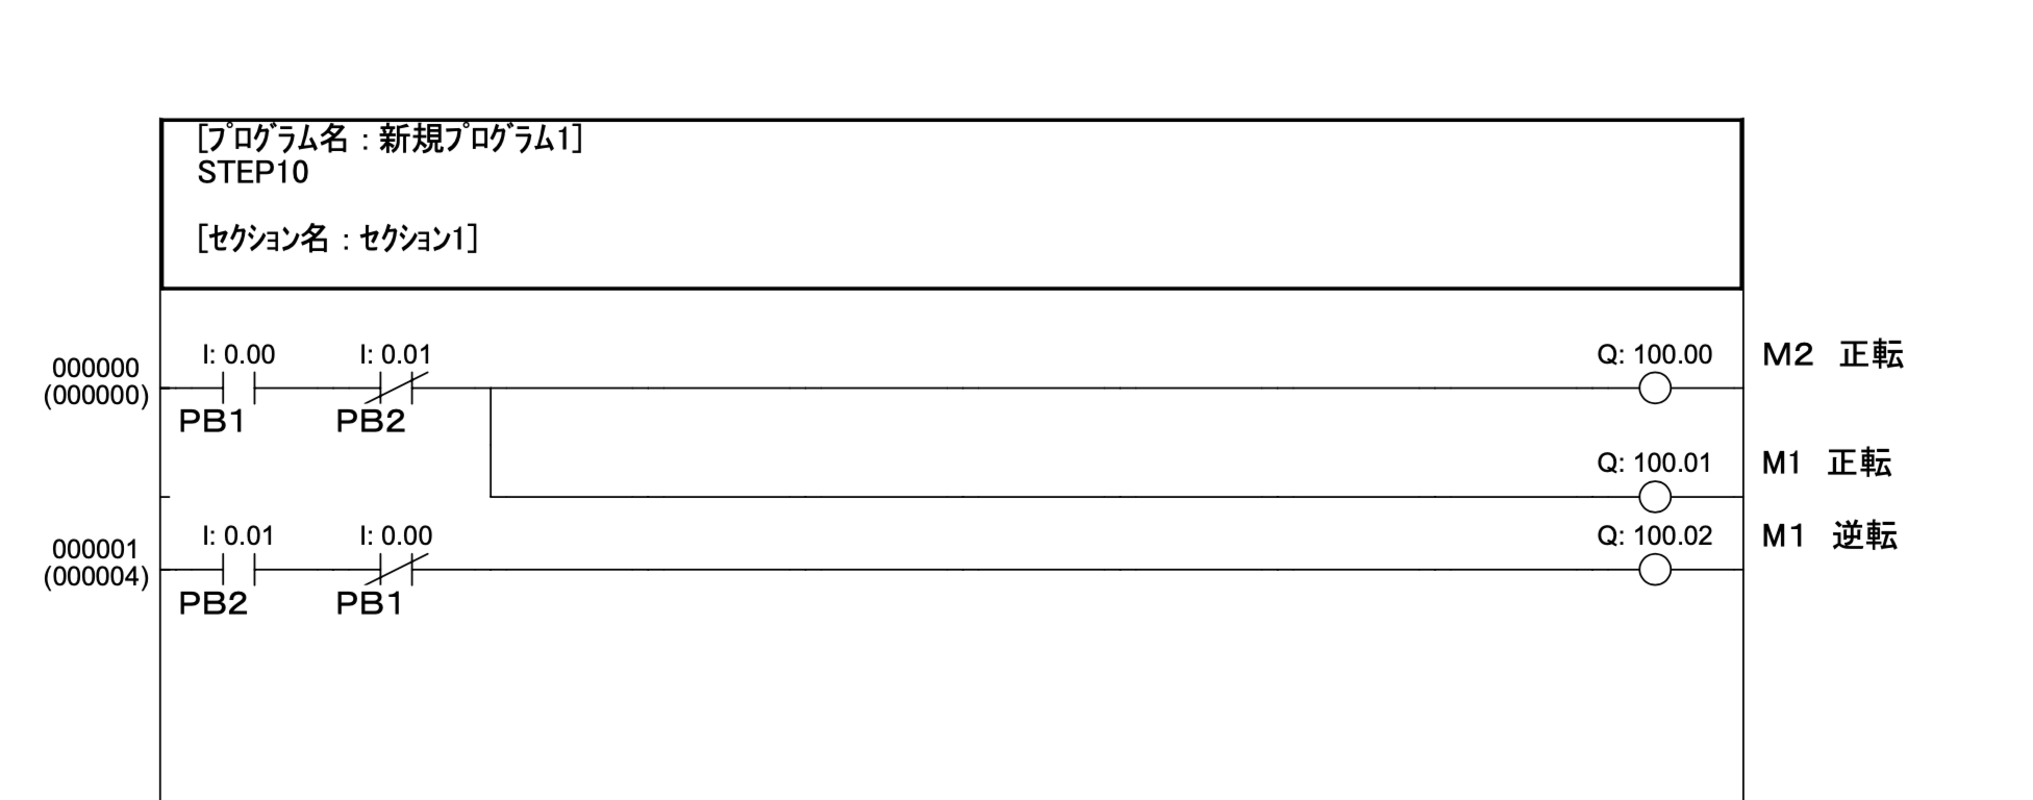
\includegraphics[clip,width=7.5cm]{picture/Step10.pdf}
    \end{center}
    \caption{STEP10のラダー図}
    \label{C:Step10}
  \end{minipage}
\end{figure}
図\ref{P:Circuit10}について説明する.押しボタンスイッチ1(PB1)が押された時,モータ1(M1),モータ2(M2)における2,4に対して出力信号が送られる.
また,押しボタンスイッチ2(PB2)が押された時,モータ1(M1),モータ2(M2)における1,3に対して出力信号が送られるが,M2の3については動線が接続されていないため
モータは回転しない.従って押しボタンスイッチ1と押しボタンスイッチ2には動作の差別化が図られている.
\par
ラダー図\ref{C:Step10}について説明する.理想動作は,押しボタンスイッチ1がONされている時,モータ1とモータ2それぞれが右移動,右回転をするとされている.また,押しボタンスイッチ2
がONされている時はモータ1だけが動作する.ただし,押しボタンスイッチ1がONされているときに押しボタンスイッチ2の入力は遮断されており,押しボタンスイッチ2がONされているときは押しボタンスイッチ2の入力は
遮断されている.これを実現するために,ラダー図上では押しボタンスイッチ1がONされ,押しボタンスイッチ2がOFFのときにM1,M2が正転するようにし,押しボタンスイッチ2がONされ,押しボタンスイッチ1がOFFの時はM1のみが逆転するようなラダー図を作成した.
\par
動作は,予想した通りに動き,回路,ラダー図が共に正しかったことがわかった.
\subsection{STEP11}
\begin{figure}[H]
  \begin{minipage}{0.38\textwidth}
    \begin{center}
      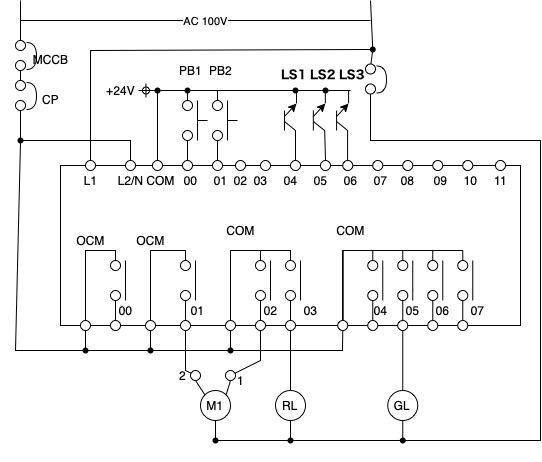
\includegraphics[clip,width=6.5cm]{picture/Circuit11.png}
    \end{center}
    \caption{STEP11の回路図}
    \label{P:Circuit11}
  \end{minipage}
  \begin{minipage}{0.58\textwidth}
    \begin{center}
      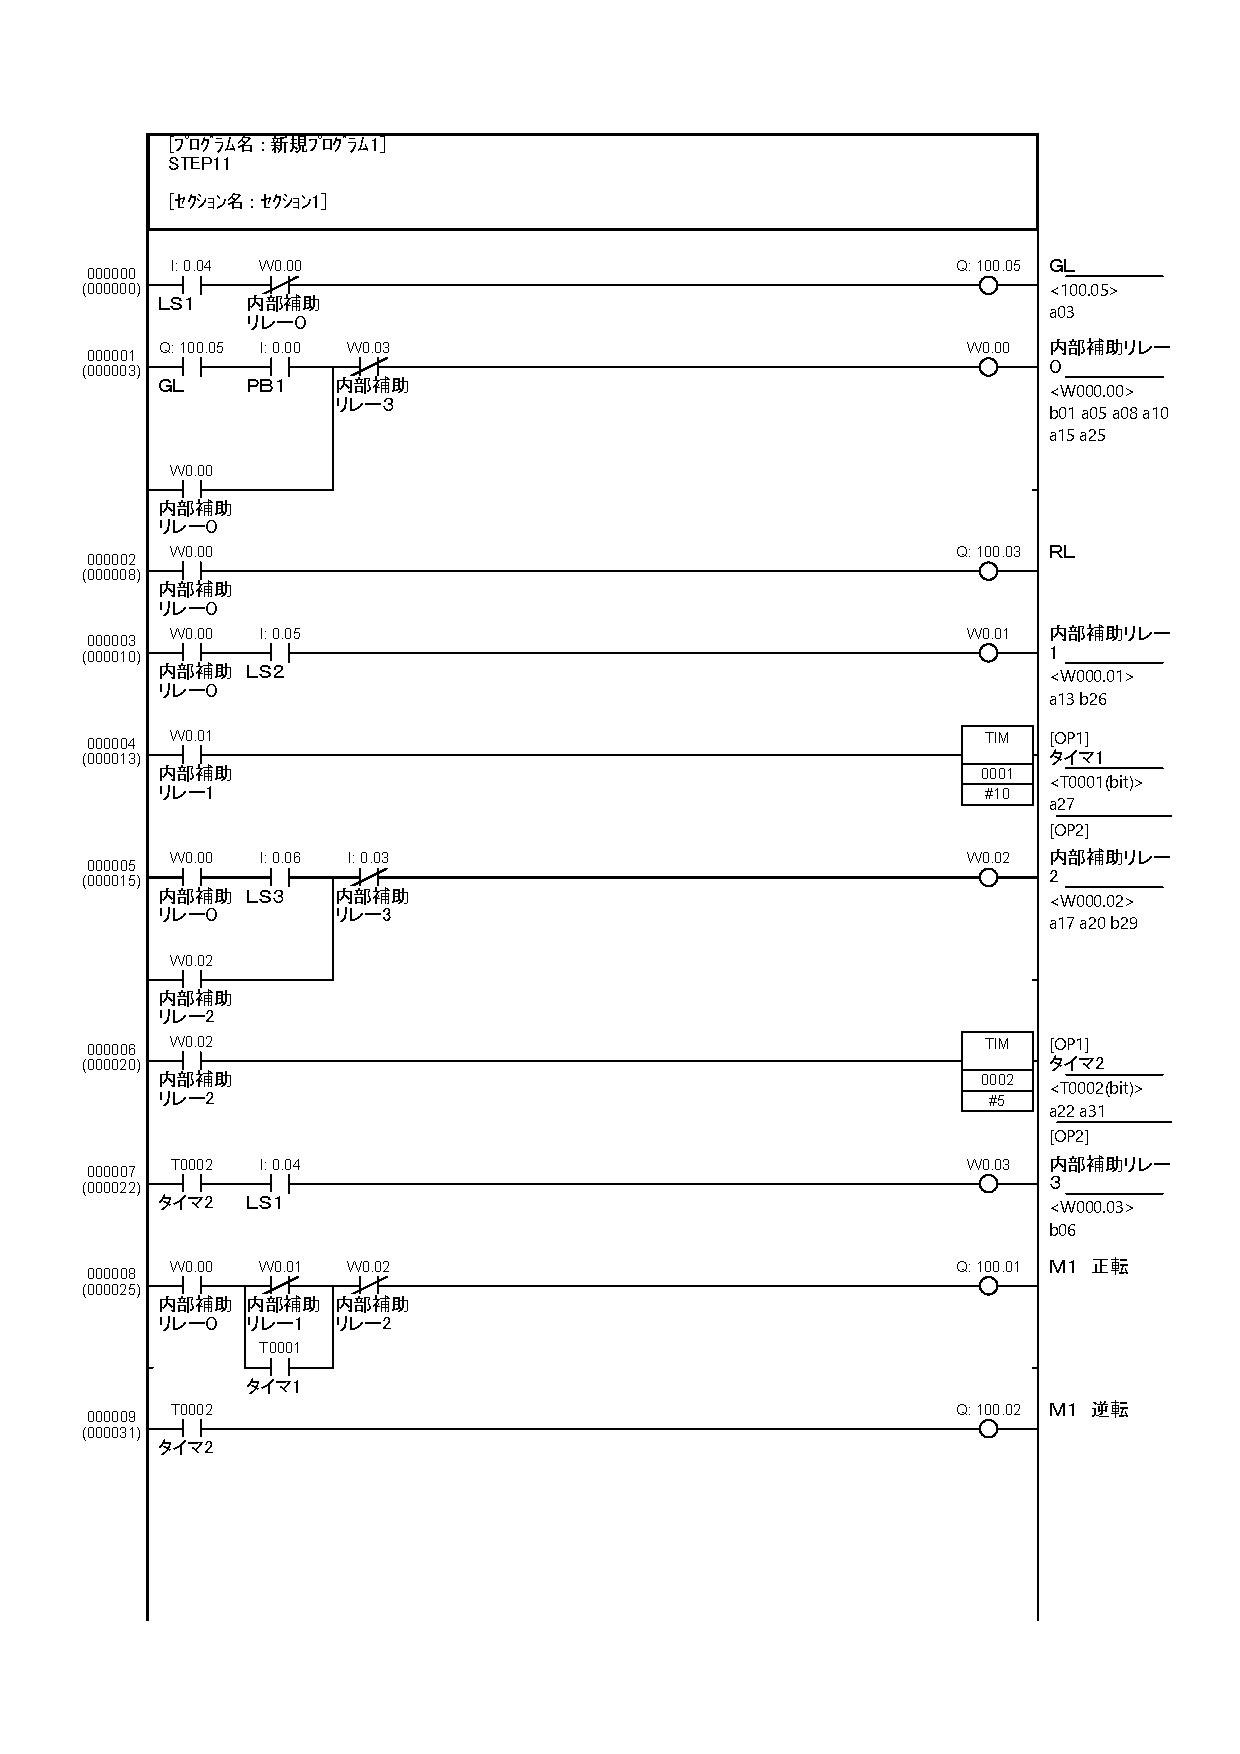
\includegraphics[clip,width=7.5cm]{picture/STEP11.pdf}
    \end{center}
    \caption{STEP11のラダー図}
    \label{C:Step11}
  \end{minipage}
\end{figure}
図\ref{P:Circuit11}について説明する.押しボタンスイッチ1(PB1)がONされた時,モータ1(M1)が動作する.センサが三つ(LS1,LS2,LS3)搭載されており,常に入力信号のチェックが行われている.
センサからの入力信号を元に,M1の回転方向が変化するよう,M1には1,2の導線をつないでいる.また,動作状態が分かりやすくなるよう,LED(RL,GL)を取り付けている. \par

ラダー図\ref{C:Step11}について説明する.理想動作は,押しボタンスイッチ1(PB1)をONした時,モータ1(M1)が正転し,センサ(LS2)がONになるとモータ1が1秒間停止する.その後,再び動作を再開し,センサ(LS3)がONになるとモータ1が0.5秒間停止する.
その後,逆回転を始め,センサ(LS1)がONになると停止する.ラダー図上において,センサ系は全てNormally Openで接続し,内部補助リレーを多く接続することで,LEDやタイマをリンクさせている.\par
動作は,予想した通りに動き,回路,ラダー図が共に正しかったことがわかった.

\section{研究課題}
\subsection{理想動作}
押しボタンスイッチ1をONすると,モータ2が正回転(CW)します.\\
押しボタンスイッチ2(停止ボタン)をONすると,LS4(センサ)のONを確認してモータ2が停止します.

\subsection{実験結果}
以下の図\ref{P:Circuit12}に作成した回路図を示し,図\ref{C:Step12}に作成したラダー図を示す.
\begin{figure}[H]
  \begin{minipage}{0.38\textwidth}
    \begin{center}
      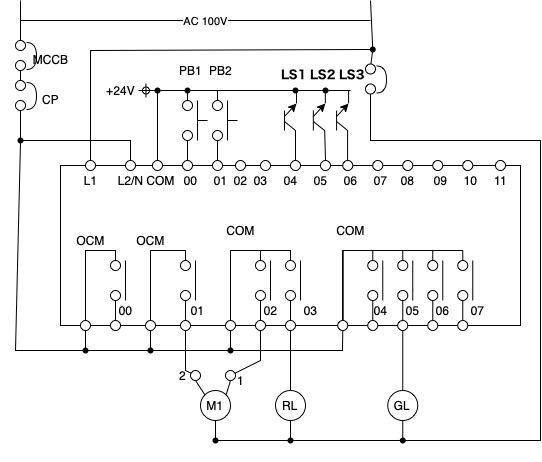
\includegraphics[clip,width=6.5cm]{picture/Circuit11.png}
    \end{center}
    \caption{STEP12の回路図}
    \label{P:Circuit12}
  \end{minipage}
  \begin{minipage}{0.58\textwidth}
    \begin{center}
      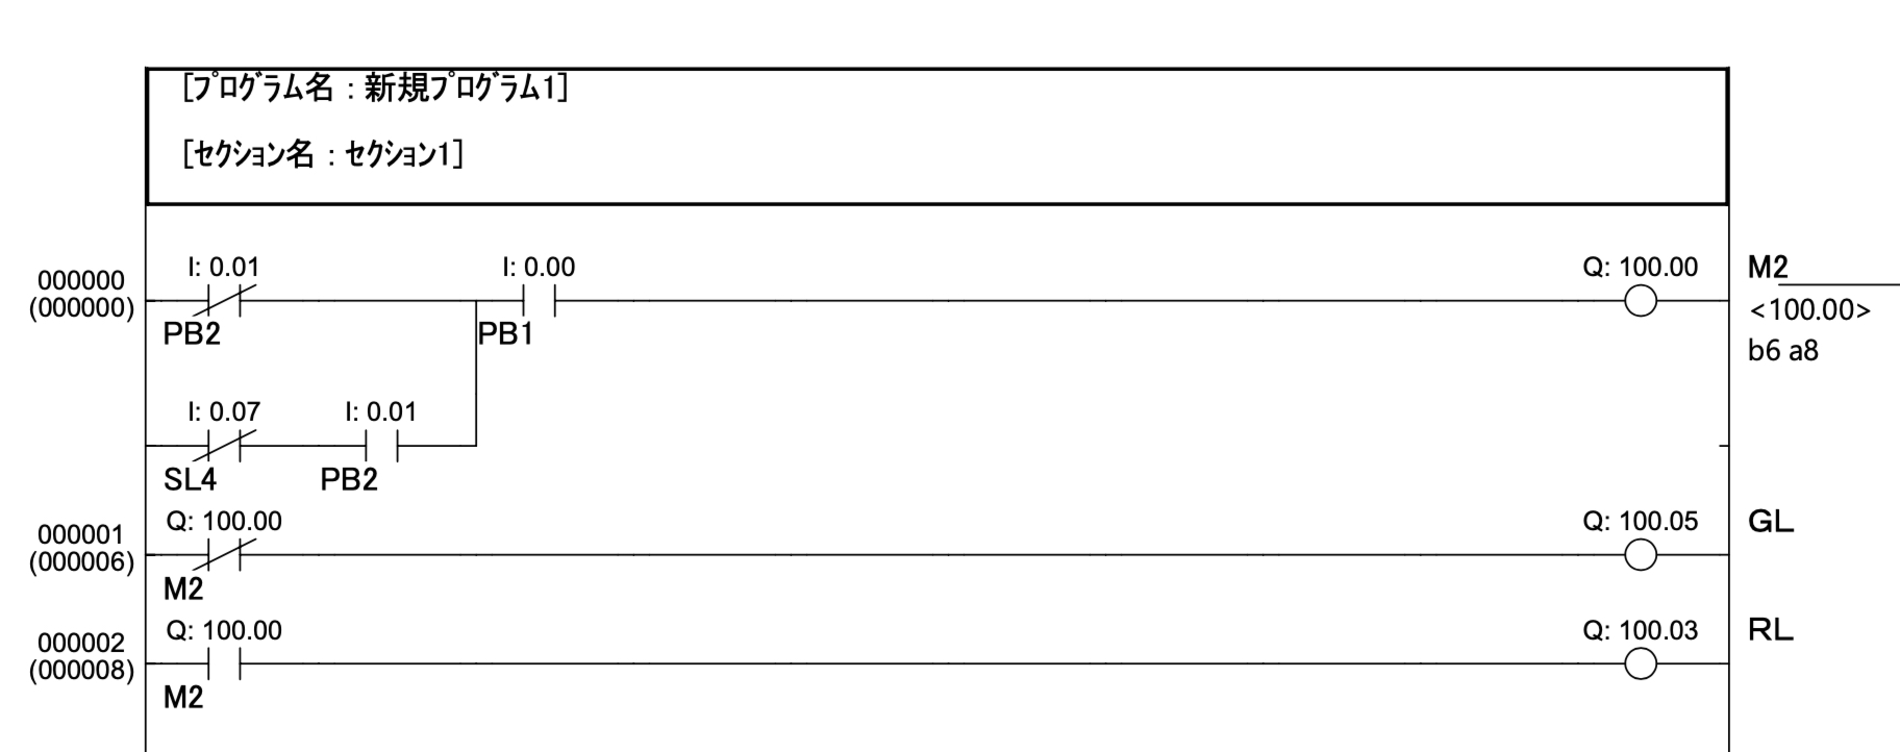
\includegraphics[clip,width=7.5cm]{picture/Step12.pdf}
    \end{center}
    \caption{STEP12のラダー図}
    \label{C:Step12}
  \end{minipage}
\end{figure}
回路図\ref{P:Circuit12}については,Step11で使用した回路と変わらない.\par
ラダー図\ref{C:Step12}について説明する.理想動作より,押しボタンスイッチ1がONされている時,モータ2は正回転する.また,押しボタンスイッチ2をONした時,
すぐには止まらずに,LS4(センサ)がONされるのを待ってから停止する.従って,モータが回転する条件が以下のようになる.
\begin{enumerate}
  \item 押しボタンスイッチ1がONされ,押しボタンスイッチ2がOFFの時 \\
  \item 押しボタンスイッチ1がONされ,押しボタンスイッチ2もONされ,SL4がOFFの時
\end{enumerate}
従って,PB2のNormally Closeは,SL4のNormally CloseとPB2のNormally OpenとのANDと,ORで接続されている.
また,モータの出力状態を受けてLEDが点灯するプログラムを作成した.\par
動作は,予想した通りに動き,回路,ラダー図が共に正しかったことがわかった.

\section{考察}
図\ref{C:Step12}に示したラダー図において,モータが回転する条件を考慮して作成した初期のラダー図から大幅な簡略化を行なった.その手順を以下に説明する.\par
条件より,$\left[PB1(NO) \& PB2(NC)\right] OR \left[SL4(NC) \& PB2(NO) \& PB1(NO)\right] OR \left[PB2(NO)\right]$のプログラムを作成した.
ここで,3つ目の条件であるPB2(NC)は一つ目の条件にも含まれており,重複が見られるため削除し,一つ目と二つ目の条件に含まれるPB1(NO)は括り出すことができるため,ORの中から括り出した.\\
このように簡略化することでプログラムを見やすくすることができ,プログラムのミスを無くすことができた.
\section{感想}

\begin{thebibliography}{99}
  \bibitem{Text} メカトロニクスシリーズ2,``プログラマブルコントローラー編【オムロン SYSMAC CPM1A仕様】'' \\
  \bibitem{JIS} 日本工業規格 JIS,``自動制御用語- 一般'',p5,4-24 \\ \url{https://kikakurui.com/z8/Z8116-1994-01.html} \\

\end{thebibliography}

\end{document}